\documentclass[tikz,border=10pt]{standalone}
\usepackage{tikz}
\usepackage{graphicx}
\usetikzlibrary{positioning,3d,shapes.misc}

\begin{document}

	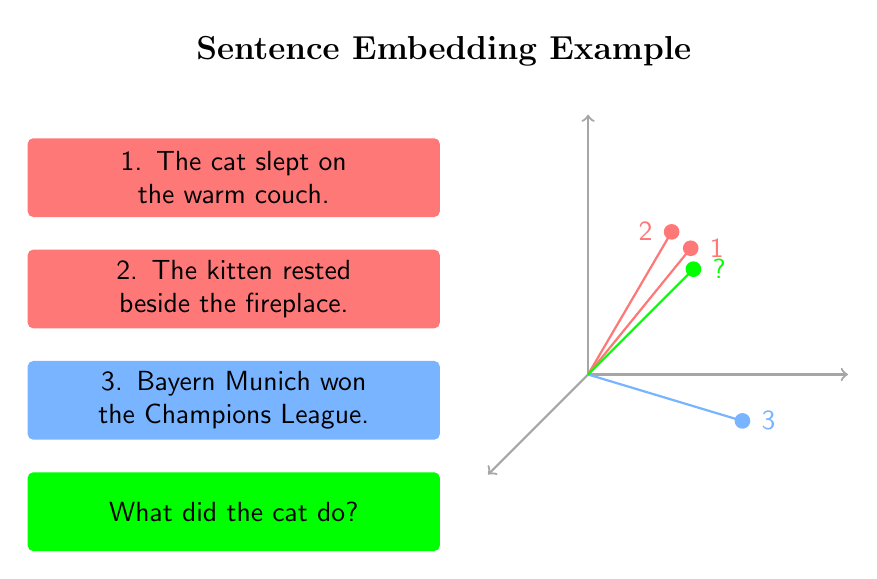
\begin{tikzpicture}[font=\sffamily]

		% Farben definieren
		\definecolor{lightred}{RGB}{255,120,120}
		\definecolor{lightblue}{RGB}{120,180,255}

		% --- Textboxen auf der linken Seite ---
		\node[rectangle, fill=lightred, rounded corners=2pt, text width=5cm, align=center, minimum height=1cm] (t1)
		{1. The cat slept on the warm couch.};
		\node[rectangle, fill=lightred, rounded corners=2pt, text width=5cm, align=center, below=0.4cm of t1, minimum height=1cm] (t2)
		{2. The kitten rested beside the fireplace.};
		\node[rectangle, fill=lightblue, rounded corners=2pt, text width=5cm, align=center, below=0.4cm of t2, minimum height=1cm] (t3)
		{3. Bayern Munich won the Champions League.};
		\node[rectangle, fill=green, rounded corners=2pt, text width=5cm, align=center, below=0.4cm of t3, minimum height=1cm] (t4)
		{What did the cat do?};


		% --- 3D Koordinatensystem ---
		\begin{scope}[xshift=4.5cm, yshift=-2.5cm, line cap=round, line join=round, thick, scale=1.5]
			% Achsen
			\draw[->, gray!70] (0,0,0) -- (2.2,0,0) node[below left]{};
			\draw[->, gray!70] (0,0,0) -- (0,2.2,0) node[left]{};
			\draw[->, gray!70] (0,0,0) -- (0,0,2.2) node[above]{};

			% Vektoren
			\draw[thick, color=lightred] (0,0,0) -- (1.1,1.3,0.6) node[circle, fill=lightred, inner sep=2pt, label={[lightred]right:1}]{};
			\draw[thick, color=lightred] (0,0,0) -- (0.9,1.4,0.5) node[circle, fill=lightred, inner sep=2pt, label={[lightred]left:2}]{};
			\draw[thick, color=lightblue] (0,0,0) -- (2.0,0.3,1.8) node[circle, fill=lightblue, inner sep=2pt, label={[lightblue]right:3}]{};
			\draw[thick, color=green] (0,0,0) -- (1.2,1.2,0.8) node[circle, fill=green, inner sep=2pt, label={[green]right:?}]{};
		\end{scope}

		% Beschriftung
		\node[font=\large\bfseries, anchor=west] at (-0.6,1.6) {Sentence Embedding Example};

	\end{tikzpicture}

\end{document}
